\documentclass[conference]{IEEEtran}
\hyphenation{op-tical net-works semi-conduc-tor}

\usepackage{float}
\usepackage{graphicx}
\usepackage{hyperref}
\usepackage{enumitem}

\begin{document}
\title{A Database Management System for a Geospatially-Enabled Interactive Game}
\author{\IEEEauthorblockN{Arturo Casillas}
\IEEEauthorblockA{\small Southern Methodist University\\
Dallas, Texas\\
Email: acasillas@smu.edu}
\and
\IEEEauthorblockN{Rene Pineda}
\IEEEauthorblockA{\small Southern Methodist University\\
Dallas, Texas\\
Email: rpinedaalvarenga@smu.edu}
\and
\IEEEauthorblockN{Volodymyr Orlov}
\IEEEauthorblockA{\small Southern Methodist University\\
Dallas, Texas\\
Email: vorlov@smu.edu}
\and
\IEEEauthorblockN{Vitaly Briker}
\IEEEauthorblockA{\small Southern Methodist University\\
Dallas, Texas\\
Email: vbriker@gmail.com}}

\maketitle

\begin{abstract}
The success of Pokémon Go\footnote[1]{Pokémon Go Wikipedia page: https://goo.gl/LeX1D3} and its predecessor, Ingress\footnote[2]{Ingress Wikipedia page: https://goo.gl/6VXFoC} demonstrates that the users of smartphones respond positively and engage with interactive technologies such as augmented reality and location services. Massive online games where players actively move around the world might impose significant technical challenges for a game designer. These issues and possible solutions have note been given enough attention in the literature. This work is based on our experience of design and implementation of geospatially-enabled interactive game and gives an overview of the available database technologies which can be used for multiplayer mobile game where device's GPS coordinates are used to locate and capture virtual tokens. 
\end{abstract}

\IEEEpeerreviewmaketitle

\section{Introduction}
Location based apps and services are becoming more and more popular. The game Pokémon Go, in particular, has gained over 44 million users and additionally incorporates augmented reality. We developed a database that can collect, store and aid in processing information for a game where players are collecting items in different tourist destinations to earn points. The game consist of players moving around the real world and collecting tokens that gradually reveal parts of a story. The data is collected from a user interface operating on their cellphones. The emphasis of this work is to design a system that can efficiently collect and store geospatially enabled data, and use a database structure to manage the game rules and possible interactions among players. 

\subsection{Previous work related to the problem}
An interesting paper by Chulmo Koo and others investigate relationship between geospatially enabled mobile game and destination satisfaction \cite{destination-engagement}. Besides, some authors argue that location-based games are positively associated with a set of beneficial health behaviors \cite{pokemon-motivation}. We found it interesting that a game can have a positive effect on tourism and person’s wellness and would like to extend research in this area.  
   Initial research in this area brought us to a paper summarizing design patterns possible with location-based games \cite{location-based-mg}. Due to time and resource limits imposed on us we decided to use on Search-and-Find pattern for our game. On the other hand, the large-scale nature of multiplayer games might generate enormous data sets. Effective handling of this data requires a sophisticated database management system \cite{data-store-issues, location-based-services}. In his thesis, Kristian Midtgård looks at the NoSQL landscape in an attempt to find the best practices and candidate databases for achieving high write throughput \cite{massive-amounts-location-data}. We've built our work on top of his research and look at other, more modern databases. 

\section{Game rules and design considerations}
\subsection{Problem statement}
As mentioned, the game consists of players exploring the real world in search of tokens. Collecting tokens raises the player’s score which will in turn reveal a segment of a story once the player’s score reaches a certain threshold. The tokens belong to different categories that correspond to different scores that must be earned and different aspects of the story that may be revealed. As such, this game relies heavily on the search-and-find mechanic as well as desires for collection, completion, and closure of narrative for player engagement \cite{game-methodology, location-based-games}. 

The story is a science fiction story that places the player in the role of an explorer. The player finds himself exploring ruins on another world that once housed an advanced civilization. The player must then find tokens that will divulge information about this lost civilization including clues as to what caused the civilization to disappear. Categories consist of Culture, Politics, Technology, and Economy and correspond to the nature of the clues the player discovers.

Given the rules, mechanics, and the location-based nature of the game, some data and database design considerations are:

\begin{enumerate}
	\item Nature of Geospatial Data. Learning data types, how they are stored, and how they may be obtained both from the player and by the player.
	\item Available DBMS. What databases and existing software packages work well with GPS data and are also capable of implementing game rules.
	\item Using Location Data. What computations can be done with GPS coordinates to enforce game rules and accomplish game mechanics such as the player interacting with geospatial objects.
	\item Database Schema. What entities and attributes are necessary to store and what portions of the game may be saved by the player.
\end{enumerate}
	
\section{High-level description of the system}
In order to be able to serve big number of requests in a timely manner and scale well with increasing number of players we need a system that will not only have a well designed, scalable database, but also other components integrated into a single, well thought architecture. Our system is built from 3 major components:

\begin{enumerate}
  \item Client-side application. We decided to support 2 major platforms that got widespread adoption: Android and iOS. For the proof-of-concept we focused on iOS. 
  \item Backend services, or middle layer. This component performs server-side operations, enforces gameplay rules and handles requests to our database. 
  \item Geospatially enabled database. Here all information regarding our players, tokens and corresponding states is being kept. 
\end{enumerate}

We use following communication protocols between these components:

\begin{enumerate}[label=\Alph*]
\item REST over HTTP. This protocol is used to send messages from the client to the server sides and back
\item SQL. We use relational database and SQL over Application Layer to transform and query our data. 
\end{enumerate}

On the client side we use Apple’s Core Location Framework to collect longitude and latitude of a player and Apple’s ARKit to place tokens around player. We calculate bearing and distance between player and a token to place tokens around given user. To uniquely identify each player we use Vendor ID.
We want our backend to support large number of requests coming from multiple players. To achieve that we use multiple copies of the identical services capable to scale up or down depending on the level of load. Luckily we do not have to think about scalability properties of our hardware since we run our services in AWS Cloud on EC2 virtual instances.  To spread load across multiple copies of the backend service we use AWS load balancer that distributes client’s requests in a round-robin fashion between EC2 instances. 
We use AWS to host our database. 
Layout of all three components are represented schematically in \autoref{schema}. 

\begin{figure}
\centering
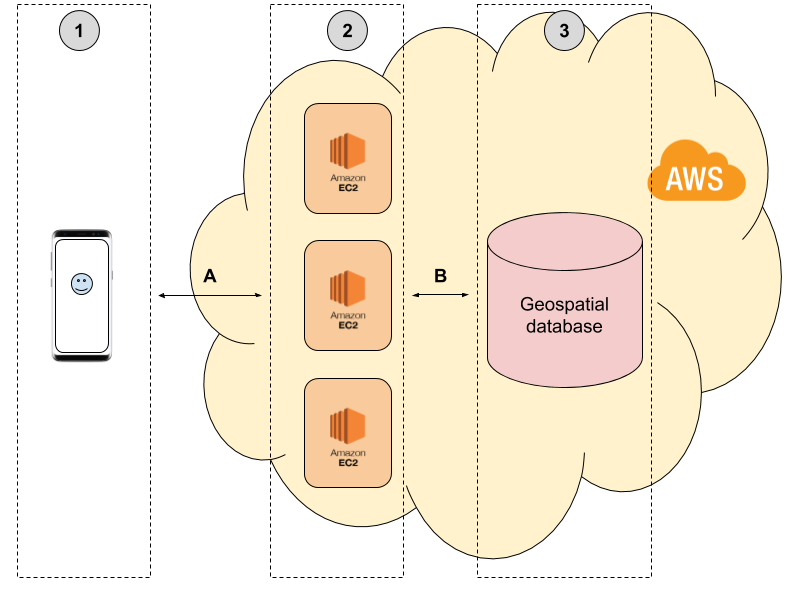
\includegraphics[width=2.5in]{imgs/systemschema.png}
\caption{Schematic layout of major components of the system}
\label{schema}
\end{figure}

\section{Choice of database}
\subsection{Representing GPS location data}

An important aspect when dealing with geospatial data is how to represent the data efficiently in order to reduce network traffic and storage requirements. A geospatial location is defined by its latitude and longitude coordinates. There are different formats in which these coordinates can be represented. The most common format for many applications (such as Google Maps and Geographical Information Systems or GIS) is the signed degrees format. The rules for this formatting are as follows:
\begin{itemize}
\item Latitudes range from -90 to 90, and longitudes from -180 to 180. 
\item South latitudes and West longitudes are preceded by a minus sign.
\item The format uses decimal places, which give the desired amount of precision. 
\end{itemize}

For example, the location of the American Airlines Center in Dallas is 32.78766352 (North Latitude) and  -96.80616344 (West Longitude).

We have two main options to represent the data in the database:
Option 1. Using the latitude and longitude data as two separate attributes, formatting them as decimal numbers, accommodating enough digits to hold the level of precision we require from the locations. 
Option 2. Using Spatial Data Types. An alternative to use numeric values for latitude and longitude is to use spatial data type, which uses the POINT type for coordinates, and geometries to represent coordinate space. This data type is specified based on the OpenGIS specification, and it has X and Y coordinate values with no separating comma: POINT (X Y). 

\subsection{Frequency of updating} 

For the purpose of supporting the gameplay, it is important to update player’s locations when they move to a new destination where collectible objects are available. While visiting tourist destinations, people travel at widely varying speeds depending on whether they are walking, riding a bike, driving, on a train, etc. Also, if there might be different locations close to each other. Therefore, it is important for people travelling at higher speeds or that are in areas with many destinations close to each other to update their location more frequently. 

Ideally, we should build a function to trigger an update after the person has moved to a new location, or some time has passed. The time threshold should not be too small to avoid many meaningless updates from non-moving people. For practical purposes, we could set the distance threshold to 50 meters and the time threshold to 5 minutes. This could change, however, depending on how the gameplay is further defined.  

It is important to create a database system that can ensure the consistency and accuracy of the data even when the information of many closely-located players is been updated frequently. 

\subsection{Location Accuracy} 

As we discussed above, latitude and longitude are more precise when they use more decimals. Using 8 decimal places would give an exact location within 1 millimeter. This could present some challenges due to the increasing volume of data stored required by the higher precision. Our project does not require this type of precision, but it needs to be sufficiently precise to identify different locations within one building. A precision of around 10 meters could be enough. This could be achieved by using 4 or 5 decimal places for our data. 

This information is important because it determines, along with the number of players, how much data is stored in the database. If the amount is very large, some sort of data compression would be necessary.

\subsection{Database Options}

\begin{enumerate}

\item MySQL: a MySQL database does not support geospatial data, using either a numeric or a spatial format. The major advantages of using this DBMS would be simplicity of the interface, and its open source nature. A major limitation could be that it only supports B+ Trees, which could impose restrictions to the storage and indexing of the data, an important component of the project. 

\item PostgreSQL: PostGIS is a spatial database extention for PostgreSQL object-relational database. It adds support for geographic objects allowing location queries to be run in SQL. The three features that PostGIS delivers to PostgreSQL DBMS are spatial types, indexes and functions such as distance, area, union, intersection, and specialty geometry. This spatial database stores and manipulates spatial objects like any other object in the database. With support for different geometry types, the PostGIS spatial database allows querying and managing information about locations and mapping.

\item MongoDB: MongoDB is a document database with an expressive query language, support for secondary indexes and easy accommodation of changes in applications. The dynamic document data model of MongoDB removes the need for a central catalog describing the structure of documents. Every document is self-describing by defining the field names internally, which comes at the cost of greater use of space. Data is stored in the BSON format, a binary encoding of JSON, which does not compress data. 
Regarding location data, MongoDB offers geospatial indexes), which allows location data to be efficiently retrieved based on longitude and latitude. Such an index is useful only if records contain other fields beside location.
 
\item Cassandra: Another popular NoSQL database is Cassandra. According to our research, however, the development of geospatial data indexing and retrieval features has been lacking for this database.  Recent research show how geohashing techniques can be used to index store data, converting the latitude/longitude information to a numeric geohash attribute and associating it to the data when being stored. However, this might make this database less attractive than the first option. 

\end{enumerate}

Our work is based on the open-sourced PostgreSQL database, integrating the capabilities of the PostGIS extension. Apart from the aforementioned advantages of using these tools, our research indicates that PostGIS is close to becoming the standard to manage geolocation data for SQL databases.  This allows us to build a database with the following capabilities:
\begin{itemize}
\item	Once the data is uploaded, use simple SQL language to run complex queries related locations, objects, and other spatial data. 
\item Scale out the database in various ways: a. Manage a very large data size because it offers multi-TB capabilities, b. Handle a large amount of concurrency from the data, c. Use table-partitioning to break large data sets down into more manageable pieces.
\item Build custom functions using a language such as Python or R, which will be very useful to program the game requirements, rules and mechanisms into the database. 
\end{itemize}

\section{Database design}

The important entities that the database must be store are player data, story-segments, token-category properties and token locations. As developers, we also need to know a player’s score in order to know what story segments the player has earned. Similarly, we need to know what tokens have already been collected in order to not allow the player to collect them again. 

\begin{figure}[h]
\centering
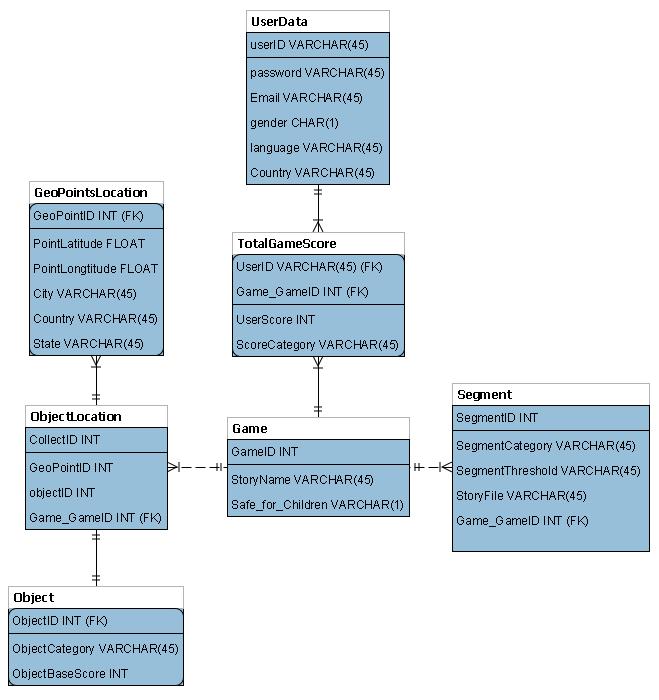
\includegraphics[width=2.8in]{imgs/MSDS7330_FinalProj_Prelim_ER2.png}
\caption{Entity Relationship Diagram of Game Database}
\label{ERD}
\end{figure}

Player information, story segment information, and information about the five categories of tokens can be stored in their own tables. There will be a central table that links these various entities via a Game-ID. This in anticipation that we may want to tell two stories in the same city. A list of geospatial points that correspond to viable latitudes and longitudes that can be used for any particular game will be stored separately from the list of geospatial points that are actually available to the player. This allows us to update the list and properties of physical geospatial points without affecting existing games and applications. A diagram of the database schema can be found above in \autoref{ERD}. 

One major consideration in choice of database schema is to what extent the game may be housed on the player’s phone and what may be streamed from the central database. The former makes data integrity more feasible while the latter makes the storage of the player’s progress more feasible. For example, knowing what tokens the player has already collected entails storing information that depends on both the player base and all of the tokens’ geospatial locations. Hence, it merits its own table the size of the number of players times the number of token locations.  As the player base increases and the game is expanded, this table will grow very rapidly in size. However, if the player holds the token locations portion of the database on his or her phone, then the information may simply be stored as an indicator on the player’s downloaded schema. An example of the schema that can be saved on the player's phone lies below in\autoref{ERDUser}. 

\begin{figure}[H]
\centering
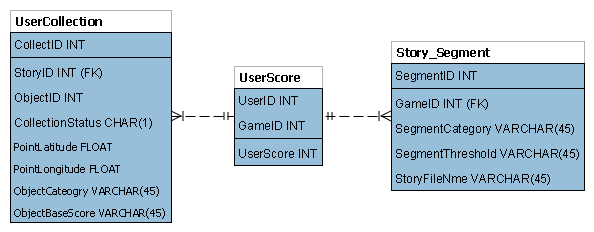
\includegraphics[width=2.7in]{imgs/MSDS7330_FinalProj_Prelim_ER2_USER.png}
\caption{ER Diagram of Database on User End}
\label{ERDUser}
\end{figure}


\section{Conclusion}
TBD

\section*{Acknowledgment}


The authors would like to thank...


\begin{thebibliography}{1}
  
\bibitem{destination-engagement}
Koo Chulmo, Choi Kyuwon, Ham Juyeon, Chung Namho. Empirical Study About the PokémonGo Game and Destination Engagement, 2018

\bibitem{pokemon-motivation}
Marquet O, Alberico C, Adlakha D, Hipp JA. Examining motivations to play Pokemon Go and their influence on perceived
outcomes and physical activity. JMIR Serious Games 2017

\bibitem{location-based-mg}
L. Lehmann, Location-Based Mobile Games. GRIN Verlag Munich Germany, 2012.

\bibitem{data-store-issues}
J. Krumm and S. A. Shafer. Data store issues for location-based services. IEEE Data Eng. Bull., 2005.

\bibitem{location-based-services}
Jensen, C., Christensen, A., Pedersen, T., Pfoser, D.,Saltenis, S. and Tryfona, N. (2001). "Location-Based Services: A Database Perspective" Proceedings of Scandinavian GIS

\bibitem{massive-amounts-location-data}
K. Midtgård. Collecting massive amounts of location data in a NoSQL database. Master of Science in Computer Science, Norwegian University of Science and Technology, 2017

\bibitem{game-methodology}
R. Dillon, "The 6-11 Framework: A new methodology for game analysis and design" presented at the Proceedings Game-On Asia Conference, Singapore, Mar., 2011.

\bibitem{location-based-games}
L. Lehman, "Location-based Mobile Games" Technical University of Berlin, unpublished, 2012.

\bibitem {PostGIS scale}
Ramsey, Pau (2017)l. Scaling PostgreSQL and PostGIS, Dec 2017. URL: http://blog.cleverelephant.ca/2017/12/postgis-scaling.html

\end{thebibliography}

\end{document}


